%%%%%%%%%%%%%%%%%%%%%%%%%%%%%%%%%%%%%%%%%%%%%%%%%%%%%%%%%%%%%%%%%%%%%%%%%%%%%%%%
% PREÁMBULO
% Este documento está configurado para ser compilado con pdflatex.
% Utiliza el estándar de artículo A4 con una sola columna.
%%%%%%%%%%%%%%%%%%%%%%%%%%%%%%%%%%%%%%%%%%%%%%%%%%%%%%%%%%%%%%%%%%%%%%%%%%%%%%%%
\documentclass[11pt, a4paper]{article}

% --- Codificación y Soporte de Idioma Español ---
\usepackage[utf8]{inputenc} % Permite escribir acentos y ñ directamente
\usepackage[T1]{fontenc}    % Codificación de fuentes moderna
\usepackage[spanish]{babel} % Soporte para español (títulos, guiones)

% --- Formato y Tipografía ---
\usepackage{times} % Fuente Times New Roman (común en reportes de ingeniería)
\usepackage[a4paper, margin=1in]{geometry} % Márgenes de 1 pulgada
\setlength{\parindent}{1em} % Indentación de párrafo
\setlength{\parskip}{0.5em} % Espacio entre párrafos

% --- Paquetes Esenciales ---
\usepackage{graphicx}   % Para insertar imágenes (tus capturas)
% Permitir cortes adecuados en URLs antes de cargar hyperref
\PassOptionsToPackage{hyphens}{url}
\usepackage[hidelinks]{hyperref} % Para URLs y referencias (sin cajas rojas)
% (url será cargado por hyperref con la opción 'hyphens')
\usepackage{caption}   
 % Mejor control sobre las captions de figuras
\usepackage{fancyhdr}   % Para cabeceras y pies de página

% --- Configuración de Cabecera ---
\pagestyle{fancy}
\fancyhf{} % Limpiar cabecera y pie
\fancyhead[L]{LIS-4052: Sistemas Distribuidos}
\fancyhead[R]{Actividad 4: RMI y gRPC}
\fancyfoot[C]{\thepage}
% Requerido por fancyhdr para evitar advertencia de altura de cabecera
\setlength{\headheight}{14pt}

%%%%%%%%%%%%%%%%%%%%%%%%%%%%%%%%%%%%%%%%%%%%%%%%%%%%%%%%%%%%%%%%%%%%%%%%%%%%%%%%
% BLOQUE DE TÍTULO
%%%%%%%%%%%%%%%%%%%%%%%%%%%%%%%%%%%%%%%%%%%%%%%%%%%%%%%%%%%%%%%%%%%%%%%%%%%%%%%%
\title{Implementación y Análisis de un Sistema de Subastas Distribuido con Java RMI y gRPC}

\author{
  \textbf{Miembros del Equipo:}\\
  Camila García Álvarez\\
  Celeste Isabel Alonso García\\
  Jesús Álvarez Sombrerero
  \vspace{1em} \\
  \textit{Departamento de Computación, Electrónica y Mecatrónica}\\
  \textit{Universidad de las Américas Puebla (UDLAP)}
}

\date{26 de octubre de 2025 \\ \vspace{1em}
   \textbf{Materia:} LIS-4052 Sistemas Distribuidos \\
    \textbf{Profesor:} José Luis Zechinelli Martini
}

%%%%%%%%%%%%%%%%%%%%%%%%%%%%%%%%%%%%%%%%%%%%%%%%%%%%%%%%%%%%%%%%%%%%%%%%%%%%%%%%
% DOCUMENTO
%%%%%%%%%%%%%%%%%%%%%%%%%%%%%%%%%%%%%%%%%%%%%%%%%%%%%%%%%%%%%%%%%%%%%%%%%%%%%%%%
\begin{document}

\maketitle
\thispagestyle{empty} % Sin cabecera/pie en la página del título

\begin{abstract}
\textbf{Resumen:} En este reporte, detallamos nuestro proceso de diseño, migración e implementación de una aplicación de subastas, transformándola de una arquitectura centralizada (MVC) a un sistema distribuido.
Para cumplir con los requisitos de la Actividad 4 y obtener las décimas extras, implementamos dos soluciones paralelas utilizando Java Remote Method Invocation (RMI) y gRPC.
Resolvimos exitosamente el desafío principal de la práctica, la sincronización de estado en tiempo real, mediante la implementación del patrón observador.
Logramos esto en RMI a través de callbacks remotos y en gRPC mediante server-side streaming.
Este documento presenta nuestro diseño, un análisis de los datos obtenidos durante nuestra experimentación (basado en la rúbrica SO6) y una comparación técnica de las ventajas y desventajas de RPC, RMI y gRPC para este caso de uso.
\end{abstract}

\newpage
\tableofcontents % Añadir una tabla de contenido
\newpage

% --- Sección 1: Objetivo ---
\section{Objetivo de la Práctica}
\label{sec:objetivo}

Nuestro objetivo en esta práctica fue doble.
Primero, aplicar los procedimientos para construir una aplicación distribuida partiendo de una versión centralizada. Para obtener las décimas extras y realizar una comparación más profunda, decidimos implementar la solución completa con dos tecnologías de middleware clave: \textbf{Java RMI} y \textbf{gRPC}.

Segundo, y como reto central de la actividad, debíamos proponer e implementar una estrategia de software robusta para resolver el problema de la falta de sincronización de datos entre múltiples clientes.
Específicamente, teníamos que asegurar que cuando un usuario propone un nuevo precio, las vistas de todos los demás clientes se actualizaran automáticamente.

Como entregable final, preparamos este reporte donde demostramos, acorde a la rúbrica SO6, nuestra capacidad para:
\begin{itemize}
    \item Diseñar y llevar a cabo una experimentación adecuada.
\item Analizar e interpretar los datos que obtuvimos (logs, comportamiento de la GUI).
\item Utilizar el juicio de ingeniería para sacar conclusiones válidas.
\end{itemize}

% --- Sección 2: Diseño de la Solución ---
\section{Diseño de la Solución}
\label{sec:diseno}

La base de nuestra práctica fue la aplicación centralizada provista, que sigue el patrón Modelo-Vista-Controlador (MVC).
En esta, \texttt{SubastaVista} maneja la GUI, \texttt{SubastaModelo} contiene la lógica de negocio y el estado, y \texttt{SubastaControlador} actúa como puente.

\subsection{Arquitectura Distribuida}
Nuestra estrategia de migración consistió en identificar el \texttt{SubastaModelo} como el componente a ser centralizado y servido.
\begin{itemize}
    \item \textbf{Servidor:} Convertimos la lógica de \texttt{SubastaModelo} en el servicio remoto.
Este se convirtió en el único componente que mantiene el estado verdadero del sistema.
\item \textbf{Cliente:} Mantuvimos las clases \texttt{SubastaVista} y \texttt{SubastaControlador} en la máquina cliente.
Modificamos el \texttt{SubastaControlador} para que, en lugar de invocar métodos locales del modelo, realizara llamadas remotas (RMI o gRPC) a nuestro servidor.
\end{itemize}

\subsection{Estrategia de Sincronización: Patrón Observador (Push)}
El problema central era que una llamada remota (ej. \texttt{agregaOferta}) del Cliente A al Servidor no tenía forma de notificar al Cliente B.
El \textit{polling} (preguntar al servidor "hay cambios?" cada 'x' segundos) nos pareció ineficiente. Por ello, nuestra solución fue implementar el \textbf{Patrón Observador (Observer Pattern)}.

El Servidor actúa como el "Sujeto" (Subject) y los Clientes como "Observadores" (Observers).
\begin{enumerate}
    \item \textbf{Registro:} Cuando un cliente se conecta, no solo lo registramos como usuario, sino que también lo "suscribimos" a las actualizaciones del servidor.
\item \textbf{Lista de Observadores:} Nuestro servidor mantiene una lista de todos los observadores suscritos (clientes conectados).
\item \textbf{Notificación (Push):} Cuando implementamos un evento de cambio de estado (como \texttt{agregaProductoALaVenta} o \texttt{agregaOferta}), el servidor itera sobre su lista de observadores y les "empuja" (push) una notificación.
\item \textbf{Actualización del Cliente:} El cliente, al recibir esta notificación asíncrona, es instruido para recargar su catálogo de productos desde el servidor, refrescando así su GUI.
\end{enumerate}

Implementamos este patrón de forma idiomática en cada tecnología:
\begin{itemize}
    \item \textbf{En RMI:} Lo implementamos mediante \textbf{Callbacks}.
Definimos una nueva interfaz remota, \texttt{ClienteCallbackRMI}, que el cliente implementa.
El cliente envía su propio stub al servidor, el cual almacenamos en un \texttt{Vector}.
Cuando hay una actualización, el servidor invoca el método \texttt{notificarActualizacion()} en cada stub de cliente.
\item \textbf{En gRPC:} Lo implementamos mediante \textbf{Server-side Streaming}.
Definimos un RPC en el \texttt{.proto} llamado \texttt{suscribirseNotificaciones} que retorna un \texttt{stream} de mensajes.
El cliente llama a este método una vez. El servidor almacena el objeto \texttt{StreamObserver} del cliente y, cuando hay una actualización, llama a \texttt{onNext()} en cada \textit{observer} para enviar la notificación.
\end{itemize}

% --- Sección 3: Pasos de Desarrollo ---
\section{Principales Pasos para Desarrollar la Solución}
\label{sec:pasos}

El desarrollo de ambas soluciones (RMI y gRPC) siguió un proceso metodológico similar, partiendo de la base de código MVC. Los pasos generales que seguimos fueron:

\begin{enumerate}
    \item \textbf{Definir el Contrato:} Primero definimos la interfaz entre cliente y servidor. Para RMI, fue una \texttt{java.rmi.Remote interface}. Para gRPC, fue el archivo \texttt{.proto}.
    \item \textbf{Implementar la Lógica del Servidor:} Adaptamos el \texttt{SubastaModelo.java} original para que implementara el contrato remoto y gestionara el estado y la lista de observadores.
    \item \textbf{Adaptar el Cliente:} Modificamos el \texttt{SubastaControlador} para que utilizara el stub (RMI o gRPC) y realizara llamadas remotas en lugar de locales.
    \item \textbf{Implementar la Sincronización:} Programamos la lógica de suscripción y notificación (callbacks en RMI, streams en gRPC) en el cliente y el servidor.
\end{enumerate}

Como parte de los requisitos de las décimas extras, los detalles técnicos, fragmentos de código y pasos específicos para \textit{cada} implementación (RMI y gRPC) se encuentran documentados en el \textbf{Anexo \ref{sec:anexo}}.

% --- Sección 4: Seguridad ---
\section{Aspectos de Seguridad en el Desarrollo}
\label{sec:seguridad}

En nuestro análisis, consideramos los aspectos de seguridad de ambas plataformas, aunque su implementación completa (como el cifrado) estaba fuera del alcance de esta práctica.

\begin{itemize}
    \item \textbf{RMI:} Encontramos que la seguridad en RMI es compleja y anticuada.
Requiere un \texttt{SecurityManager} y archivos de políticas (\texttt{.policy}) para definir permisos, lo cual es verboso.
La funcionalidad de \texttt{codebase} es una vulnerabilidad conocida si no se configura adecuadamente, y la comunicación por defecto no está cifrada.
\item \textbf{gRPC:} En contraste, gRPC está construido sobre HTTP/2 y promueve la seguridad como una característica central.
Se integra nativamente con SSL/TLS para cifrar toda la comunicación.
Para nuestras pruebas, utilizamos \texttt{usePlaintext()}, pero reconocemos que habilitar el cifrado en producción es trivial.
Además, gRPC soporta mecanismos de autenticación modernos, como tokens JWT.
\end{itemize}

% --- Sección 5: Presentación de Datos e Interfaz ---
\section{Presentación de los Datos: Interfaz del Sistema}
\label{sec:interfaz}

Decidimos no modificar la interfaz de usuario (\texttt{SubastaVista.java}) visualmente, ya que el reto de la práctica era de backend y arquitectura, no de frontend.
La GUI sigue presentando las cuatro zonas funcionales descritas en las instrucciones:
\begin{enumerate}
    \item \textbf{Iniciar sesión:} Captura del nombre de usuario.
\item \textbf{Poner producto a la venta:} Nombre del producto y precio inicial.
    \item \textbf{Obtener lista de productos:} Lista de productos y precio actual.
\item \textbf{Hacer una oferta:} Monto ofrecido.
\end{enumerate}

El cambio fundamental que logramos no es visual, sino funcional.
Gracias a nuestra solución de sincronización (callback/stream), la "Zona de lista de productos" y el "Precio actual" ahora se actualizan de forma reactiva.
Cuando un cliente B realiza una oferta, nuestro servidor envía la notificación. El cliente A la recibe y su controlador recarga la lista y el precio, reflejando el nuevo estado del sistema sin intervención del usuario.

% --- Sección 6: Demostración de Ejemplos y Análisis (SO6) ---
\section{Demostración de Ejemplos y Análisis (SO6)}
\label{sec:demo}

Acorde a la rúbrica SO6 ("Diseño de experimentos" y "Análisis de datos"), diseñamos un experimento para validar nuestra solución al problema de sincronización.

\subsection{Diseño del Experimento}
El diseño experimental que aplicamos fue idéntico para RMI y gRPC, para poder comparar los resultados:
\begin{enumerate}
    \item \textbf{Inicio:} Lanzamos la aplicación del Servidor.
    \item \textbf{Conexión Cliente A:} Iniciamos un cliente (ej. "Cliente 1: Camila") y nos conectamos. Verificamos en el servidor que se registra la conexión y la suscripción.
    \item \textbf{Conexión Cliente B:} Iniciamos un segundo cliente (ej. "Cliente 2: Celeste") y nos conectamos. Verificamos que el servidor registra al segundo suscriptor.
    \item \textbf{Acción (Cliente A):} El Cliente A pone un producto a la venta (ej. "Impresora" por 3500).
    \item \textbf{Verificación (Cliente B):} Verificamos que la GUI del Cliente B se actualiza \textit{automáticamente}, mostrando el nuevo producto "Impresora" y su precio, sin haber presionado ningún botón.
    \item \textbf{Acción (Cliente B):} El Cliente B realiza una oferta por la "Impresora" (ej. 3600).
    \item \textbf{Verificación (Cliente A):} Verificamos que la GUI del Cliente A actualiza el precio actual de la "Impresora" a 3600, de nuevo, sin acción manual.
\end{enumerate}

\subsection{Análisis de Datos (SO6)}
El experimento fue un éxito en ambas plataformas.
\textbf{Los datos principales} que obtuvimos fueron los logs de las terminales y las capturas de pantalla de las GUI.

Como se demuestra en las capturas de pantalla detalladas en el \textbf{Anexo \ref{sec:anexo}} (ver Figuras \ref{fig:rmi_vender_term}, \ref{fig:rmi_oferta_gui} y \ref{fig:grpc_full}), los logs del servidor y del cliente confirman la recepción de notificaciones asíncronas (la línea "CALLBACK RECIBIDO" en RMI y los logs de "Enviando notificación" en gRPC).
Los datos de la GUI (específicamente la GUI del Cliente 2 en la Fig. \ref{fig:grpc_full} y el callback en la Fig. \ref{fig:rmi_vender_term}) validan inequívocamente que nuestra implementación del patrón observador resolvió el problema de sincronización.
% --- Sección 7: Análisis Comparativo ---
\section{Análisis y Comparación: RPC, RMI y gRPC}
\label{sec:comparacion}

Tal como lo solicita la práctica, realizamos un análisis comparativo entre las tecnologías, suponiendo un RPC tradicional.

\begin{itemize}
    \item \textbf{RPC (Tradicional):}
    \begin{itemize}
        \item \textbf{Ventajas:} Es el concepto más simple y es agnóstico al lenguaje (si usa un IDL).
\item \textbf{Desventajas:} Es un paradigma puramente síncrono (solicitud-respuesta).
Resolver el problema de sincronización de esta práctica habría requerido \textit{polling} (el cliente preguntando "¿hay cambios?" cada segundo).
Consideramos que esto es altamente ineficiente, genera alta latencia y no escala.
    \end{itemize}
    
    \item \textbf{Java RMI (Implementado):}
    \begin{itemize}
        \item \textbf{Ventajas:} Su integración con Java es nativa.
Nos permitió pasar objetos Java serializables completos. El patrón de callback fue una solución natural y elegante para nosotros dentro de un ecosistema puramente Java.
\item \textbf{Desventajas:} Es una tecnología legada, limitada exclusivamente a Java.
Su configuración (\texttt{rmiregistry}, \texttt{codebase}, políticas de seguridad) nos pareció anticuada y verbosa en comparación con gRPC.
\end{itemize}
    
    \item \textbf{gRPC (Implementado):}
    \begin{itemize}
        \item \textbf{Ventajas:} Es una tecnología moderna de alto rendimiento (HTTP/2, Protocol Buffers).
Es agnóstica al lenguaje (definida por \texttt{.proto}).
Su soporte nativo para \textbf{streaming} (unidireccional y bidireccional) fue la herramienta perfecta para este caso de uso.
Nos permitió una comunicación asíncrona y reactiva de forma muy eficiente.
\item \textbf{Desventajas:} Requiere un paso de compilación/generación de código. La gestión de la comunicación asíncrona (streams, observadores) añadió una capa de complejidad al código cliente que no tuvimos con RMI.
    \end{itemize}
\end{itemize}

% --- Sección 8: Conclusiones ---
\section{Conclusiones (Síntesis SO6)}
\label{sec:conclusiones}

Hemos cumplido en su totalidad los objetivos de la práctica.
Logramos migrar exitosamente la aplicación MVC centralizada a dos arquitecturas distribuidas funcionales, implementando la solución en RMI y gRPC.

La \textit{síntesis de la información} (rúbrica SO6) que obtuvimos de nuestros experimentos (Sección \ref{sec:demo} y Anexo \ref{sec:anexo}) nos permite concluir que el problema de sincronización de estado fue resuelto exitosamente en ambas plataformas.
Nuestra estrategia del patrón observador fue validada: los callbacks de RMI y los streams de gRPC demostraron ser mecanismos eficaces para "empujar" (push) las actualizaciones de estado a los clientes en tiempo real.

Aplicando nuestro \textit{juicio de ingeniería} (rúbrica SO6), concluimos que \textbf{gRPC es la solución tecnológicamente superior}.
Aunque nuestra implementación de RMI fue funcional y elegante dentro de su ecosistema cerrado, gRPC nos ofreció una solución más robusta, de mayor rendimiento e interoperable, cuyo soporte nativo para streaming se alinea perfectamente con los requisitos de las aplicaciones distribuidas modernas y reactivas.

\newpage
% --- Anexo para Puntos Extra ---
\appendix

\section{Anexo: DECIMAS EXTRAS (Implementación y Evidencia)}
\label{sec:anexo}

Para la obtención de las décimas extras, nuestro equipo implementó la aplicación completa en \textbf{ambas} plataformas (RMI y gRPC).
A continuación, detallamos los pasos de implementación y presentamos la evidencia experimental (capturas de pantalla) que demuestra el funcionamiento de ambas soluciones.

\subsection{Implementación RMI}
Seguimos los siguientes pasos para la versión de RMI:
\begin{enumerate}
    \item \textbf{Definición de Interfaces:} Creamos dos interfaces \texttt{java.rmi.Remote}: \texttt{SubastaServidorRMI} (para las operaciones principales: ofertar, registrar, etc.) y \texttt{ClienteCallbackRMI} (con un solo método, \texttt{notificarActualizacion()}).
\item \textbf{Serialización:} Modificamos las clases de datos \texttt{InformacionProducto} e \texttt{InformacionOferta} para que implementaran \texttt{java.io.Serializable}.
\item \textbf{Implementación del Servidor:} Creamos \texttt{SubastaModeloRMI} extendiendo \texttt{UnicastRemoteObject} e implementando \texttt{SubastaServidorRMI}. Añadimos un \texttt{Vector<ClienteCallbackRMI>} para gestionar los callbacks.
\item \textbf{Implementación del Cliente:} Modificamos el \texttt{SubastaControladorRMI} para buscar el stub del servidor en \texttt{rmiregistry}.
El cliente también implementó la interfaz de callback y se registró a sí mismo en el servidor al conectarse, enviando su propio stub.
\end{enumerate}

\subsection{Implementación gRPC}
Para la versión de gRPC, el proceso fue:
\begin{enumerate}
    \item \textbf{Definición de Contrato (IDL):} Creamos el archivo \texttt{subasta.proto}. En él, definimos los mensajes (ej. \texttt{OfertaRequest}, \texttt{Producto}) y los servicios (\texttt{rpc AgregaOferta}).
\item \textbf{Definición del Stream:} El paso crucial fue definir el stream para las notificaciones: \texttt{rpc suscribirseNotificaciones(Empty) returns (stream NotificacionUpdate);}.
\item \textbf{Generación de Código:} Usamos Gradle y el plugin de \texttt{protobuf} para generar el código stub de Java.
\item \textbf{Implementación del Servidor:} Creamos \texttt{SubastaServicioImpl} extendiendo la clase base generada por gRPC.
Migramos la lógica del modelo aquí, incluyendo un \texttt{ConcurrentHashMap} para almacenar los \texttt{StreamObserver} de los clientes suscritos.
\item \textbf{Implementación del Cliente:} Creamos \texttt{ClienteGPRC}, que instancia un \texttt{ManagedChannel} para conectarse al servidor.
El \texttt{SubastaControladorGPRC} usa el stub bloqueante para acciones (como ofertar) y el stub asíncrono para suscribirse al stream de notificaciones en un hilo separado.
\end{enumerate}

\subsection{Evidencia Experimental RMI}
Las siguientes figuras demuestran el funcionamiento de nuestra implementación RMI.
\begin{figure}[h!]
    \centering
    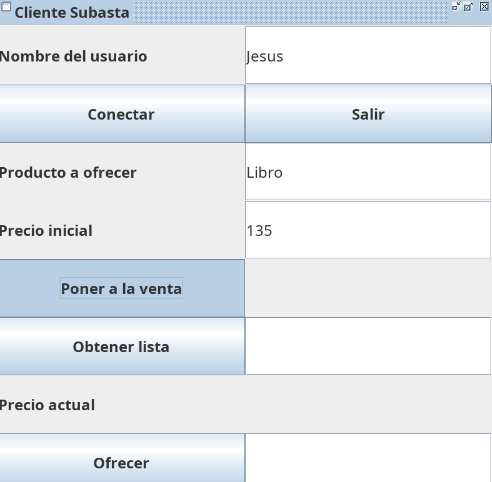
\includegraphics[width=0.7\linewidth]{media/rmi-screenshots/Sell-Item-Client1.png}
    \caption{RMI: Cliente 1 ("Jesus") poniendo a la venta un "Libro" por 135.}
    \label{fig:rmi_vender_gui}
\end{figure}

\begin{figure}[h!]
    \centering
    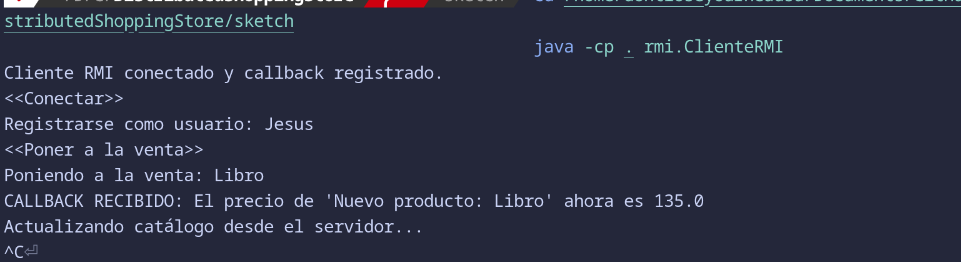
\includegraphics[width=0.9\linewidth]{media/rmi-screenshots/Sell-Item-Terminal-Client-1.png}
    \caption{RMI: Terminal del Cliente 1. La línea "CALLBACK RECIBIDO" demuestra que el servidor notificó exitosamente al cliente sobre el nuevo producto.}
    \label{fig:rmi_vender_term}
\end{figure}

\begin{figure}[h!]
    \centering
    \begin{minipage}{0.48\textwidth}
        \centering
        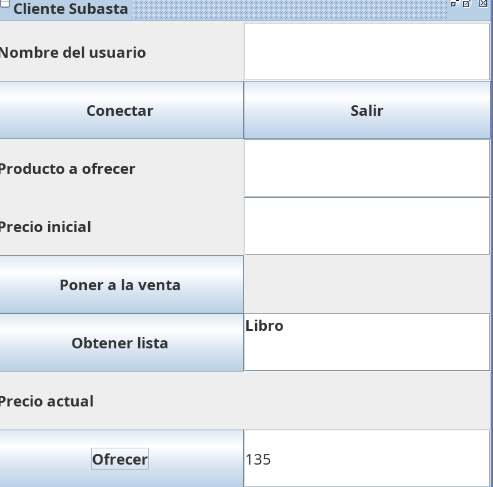
\includegraphics[width=\linewidth]{media/rmi-screenshots/Offer-Client2.png}
        \caption{RMI: Cliente 2 visualiza el 
"Libro" y prepara una oferta de 135.}
        \label{fig:rmi_oferta_gui}
    \end{minipage}\hfill
    \begin{minipage}{0.48\textwidth}
        \centering
        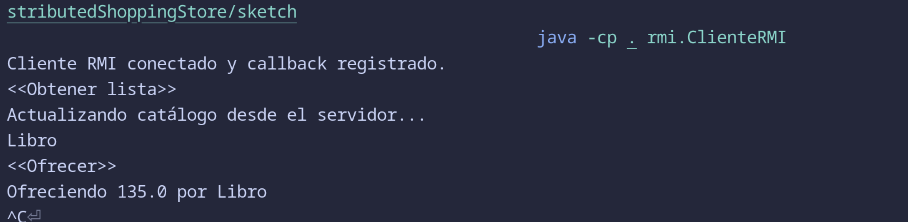
\includegraphics[width=\linewidth]{media/rmi-screenshots/Offer-Terminal-Client2.png}
        \caption{RMI: Terminal del Cliente 2, registrando la acción "Ofrecer".}
        \label{fig:rmi_oferta_term}
    \end{minipage}
\end{figure}

\subsection{Evidencia Experimental gRPC}
La siguiente figura captura la demostración completa de nuestra implementación gRPC, mostrando al servidor y dos clientes interactuando.
\begin{figure}[h!]
    \centering
    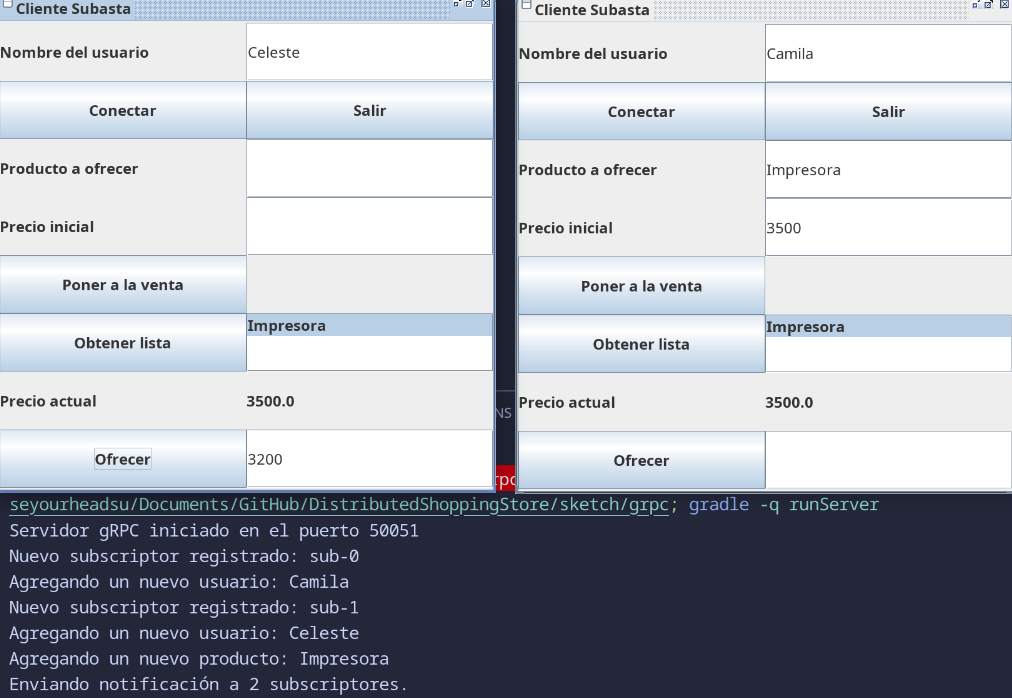
\includegraphics[width=1.0\linewidth]{media/grpc-screenshots/Two-Clients+Server-Output.png}
    \caption{gRPC: Demostración completa. El servidor (abajo) registra a "Camila" y "Celeste" . Camila (derecha) vende una "Impresora" . El servidor envía la notificación y la GUI de Celeste (izquierda) se actualiza automáticamente .}
    \label{fig:grpc_full}
\end{figure}


% --- Referencias ---
\newpage

\begin{thebibliography}{9}

\bibitem{tanenbaum}
A. S. Tanenbaum and M. Van Steen,
\textit{Distributed Systems: 
Principles and Paradigms (4th Edition)}.
Pearson, 2024.

\bibitem{coulouris}
G. Coulouris, J. Dollimore, T. Kindberg, and G. Blair,
\textit{Distributed Systems: Concepts and Design (5th Edition)}.
Addison-Wesley, 2011.

\bibitem{grpc_docs}
The gRPC Authors, "gRPC Documentation: Core Concepts, Architecture and Lifecycle."
\url{https://grpc.io/docs/what-is-grpc/core-concepts/}
[Consultado: 25 de octubre de 2025].
\bibitem{oracle_rmi}
Oracle Corporation, "Java RMI Documentation: An Overview."
\url{https://docs.oracle.com/javase/8/docs/technotes/guides/rmi/index.html}
[Consultado: 25 de octubre de 2025].

\end{thebibliography}

\end{document}